\documentclass[12pt]{beamer}
\usetheme{Boadilla}
\usepackage{graphicx}
\usepackage{algorithm2e}
\graphicspath{{images/}}
\title{CMPT 155: Computer Applications for Life Sciences}
\subtitle{Lecture 10: Discrete Probability}
\author{Ivan E. Perez}
\institute{}
\date{February 11, 2022}
\usepackage{booktabs} % Allows the use of \toprule, 
\usepackage{appendix}
\usepackage{enumerate,multicol}
\usepackage{amsmath, amssymb, amsthm}
\usepackage{tikz}
\usepackage{amsxtra}
\usepackage{emoji}
\setemojifont{TwemojiMozilla}
% !TeX program = lualatex
\begin{document}
	
	\begin{frame}
		\titlepage
	\end{frame}
	
	\begin{frame}
		\frametitle{Presentation Outline}
		\tableofcontents
	\end{frame}
	\section{Homework \& Administrative}
	
	\begin{frame}
		\frametitle{Homework \& Administrative Schedule}
		\begin{itemize}
			\item Homework 2 Due: Tuesday, February $22^{\text{nd}}$ at 6pm
			\item Homework 3 Due: Tuesday, March $1^{\text{st}}$ at 6pm
			\item First Midterm Review:  Wednesday, March $2^{\text{nd}}$
			\item First Midterm Exam: Friday, March, $4^{\text{th}}$
			
		\end{itemize}
	\end{frame}
	\begin{frame}
		\begin{itemize}
			\item Event - 
			\item Outcome 
			\item Probability
			\item Sample Space 
		\end{itemize}	
	\end{frame}		
	\begin{frame}
		\frametitle{Fundamentals of Probability}
		Discrete probability is about measuring the subset of outcomes that satisfy the restriction amongst a broader set of outcomes.\\
		\textbf{Some definitions:}
		\begin{itemize}
			\item Event:
			\begin{itemize}
				\item An observation (e.g., coin flip, card draw, dice roll)
			\end{itemize}
			\item Outcome: 
			\begin{itemize}
				\item Result of an event (e.g., Heads/Tails(H/T), King of Hearts (K$\heartsuit$), [1,6] )
			\end{itemize}
			\item Probability:
			\begin{itemize}
				\item ``Chance" of the occurrence of an event. (BOUNDED BETWEEN 0 and 1)
			\end{itemize}
			\item Sample Space
			\begin{itemize}
				\item Set of all possible outcomes of an experiment. (e.g., H/T, [1,6])
			\end{itemize}
		\end{itemize}
	\end{frame}

	\begin{frame}
		\frametitle{Some more Definitions}
		\begin{itemize}
			\item Independent Events:
			\begin{itemize}
				\item An event is called independent IF the outcome of one event does not influence the outcome of the other
		\end{itemize}
		 \item Mutually Exclusive Events/Outcomes:
		 	\begin{itemize}
		 		\item Outcomes of Events that annoc result in observing multiple outcomes at the same time. 
		 	\end{itemize}
		\end{itemize}
	\end{frame}
	\begin{frame}
		\frametitle{Priori Probability}
		The PROBABILITY of an Event(s) occuring is the COUNT of Event(s) of Interest divided by the Sample Space (i.e., the set of all possible outcomes) \\Using  notation using a coinflip:
		$$p(H) = \frac{\text{H}}{\text{H} + \text{T}} = \frac{1}{2}$$
		We can also compute the probability of rolling a \emoji{four} on a 6-sided die:
		$$p\left(\text{\emoji{four}}\right) = \frac{\text{\emoji{four}}}{\text{\emoji{one},\emoji{two},\emoji{three},\emoji{four},\emoji{five},\emoji{six}}} = \frac{1}{6}  $$
	\begin{itemize}
		\item Priori Probabilities can be computed \textit{without} experimentation.
		\item Games (rolling dice)
		\item Examples: Lottery Odds, Trading card rarity odds, poker/blackjack odds.
	\end{itemize}
	\end{frame}
	\begin{frame}
		\frametitle{Empirical Probability}
		The PROBABILITY of an Event(s) occurring is the COUNT of Event(s) of Interests divided by the total COUNT of Events observed
		\\Using notation watching 3 people enter the subway out of 10 people. 
		$$ p(\text{`Enter the Subway'}) = \frac{3}{10}$$ 
		\begin{itemize}
			\item Computed from observations or event occurrences. 
			\item Examples: Surveys, Store visits, Empirical Experiments
		\end{itemize}
		\end{frame}
	\begin{frame}
		\frametitle{Example 1: SimpleProbability.xlsx}
		\begin{enumerate}
			\item Download \textit{`SimpleProbability.xlsx'}
			\item Compute the \textit{proportions} for each set of families with 0,1,\ldots,7 children.
			\item Answer the following questions:
			\begin{itemize}
				\item Compute the probability that a family selected in this study will have \textbf{no} children?
				\item Compute the probability that a family selected in this study will have \textbf{at least 4} children?
			\end{itemize}
	\end{enumerate}
	\end{frame}
	\begin{frame}
		\frametitle{Example  1: Solution Picture}
		\begin{center}
			\includegraphics[width=0.9\textwidth]{Example1.png}
		\end{center}
	\end{frame}
	\begin{frame}
		\frametitle{What have we noticed about Probability so far?}
		\begin{enumerate}
			\item Probabilities of mutually exclusive events can be added together.
			\item The sum of the probabilities of all possible mutually exclusive events will always be \textbf{1}.
		\end{enumerate}
	\end{frame}
	\begin{frame}
		\frametitle{Exercise 1: Probability of Rolling Fair Dice}
		On a new spreadsheet layout all the possible outcomes of two rolls of a fair die.\\
		Compute the following probabilities:
		\begin{itemize}
			\item outcome of the dice roll will add up to 7.
			\item outcome of the dice roll will add up to 8 or more.
		\end{itemize}
	\end{frame}
	\begin{frame}
		\frametitle{Exercise 1: Solution}
		\begin{enumerate} 
			\item Begin by filling Column A with the range of values that two dice can take
			\item In column B list the ways each value can be observed by the dice, (e.g., 2 = snake eyes, or (1,1)) 
			\item In Column C count the different ways each value can be observed by the dice.
			\item In Column D compute the probability of each outcome by dividing count of the ways each outcome can be observed by the total count of all the different outcomes.
		\end{enumerate}			
		To compute probability ranges:
		\begin{itemize}
			\item  outcome of the dice roll will add up to 7.
			\begin{itemize}
				\item See Cell D7
			\end{itemize}
			\item outcome of the dice roll will add up to 8 or more.
			\begin{itemize}
				\item Add up the computed probabilities in cells D8:D12
			\end{itemize}
		\end{itemize}
	\end{frame}
	\begin{frame}
		\frametitle{Exercise 1: Solution (continued)}
		\begin{center}
			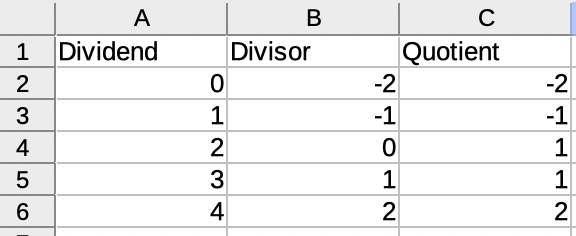
\includegraphics[width=0.9\textwidth]{Exercise1Soln.png}
		\end{center}
	\end{frame}
	\begin{frame}
		\frametitle{Exercise 2a: Binomial Modelling of Emergency Room Arrivals}
		\begin{enumerate}
			\item Layout a spreadsheet that has all the possible outcomes of a visit by three people to an emergency room.
			\item Compute the following probabilities out of three arrivals:
			\begin{itemize}
				\item \textbf{No} emergencies.
				\item \textbf{One} emergency.
				\item \textbf{Two} emergencies.
				\item \textbf{Three} emergencies.
			\end{itemize}
		\end{enumerate}
	\end{frame}
	\begin{frame}
		\frametitle{Exercise 2a: Solution}
		\begin{enumerate}
			\item Create a table that will hold all the possible order of people arriving to the emergency room
			\begin{itemize}
				\item Add the headers for arrivals 1,2, and 3 in cells A1:C1.
				\item In Cells A2:C9 write out all the possible sequences of arrivals.
			\end{itemize}
			\item Create a table that counts the \textit{ways} each emergency count is observed.
			\begin{itemize}
				\item In Cells D1:F1, add the headers for:
					\begin{enumerate}
						\item The Count of Emergencies for each case of arrivals,
						\item Count of ways to get to each case of arrivals,
						\item The Proportion/Probability of each case of arrivals.
					\end{enumerate}
			\end{itemize}
			\item In Cells D2:D5 list the emergencies count for each case.
			\item In Cells E2:E5 list the count of ways to get to each emergency case.
			\item In Cells F2:F5 compute the proportion of ways that get to the case against out of the total ways.
		\end{enumerate}
	\end{frame}
	\begin{frame}
		\frametitle{Exercise 2a: Solution (continued)}
			\begin{center}
				\includegraphics[width=0.9\textwidth]{Exercise2aSoln.png}
			\end{center}
		In the Next Exercise (2b), let's try using \textit{Emipirical} Probabilities based on data observed by a local hospital.
	\end{frame}
	\begin{frame}
		\frametitle{Exercise/Example 2b: Emergencies \textit{Empirical}}
		\begin{enumerate}
			\item Download \textit{Emergencies.xlsx}
			\item In Sheet2, Cells B12 and B13 compute the \textit{Empirical} probability of an Emergency and an Other (non-emergency) using the data.
			\item Using these computed probabilities fill in the probabilities of each independent event in Cells D3:F10.
			\item In Cells H3:H10 fill in the count of the number of emergencies in each of the listed sequence of outcomes. 
			\item Lets stop here and we will learn about the `Law of Independence' to compute the Final probabilities in cell G3:G10. 
		\end{enumerate}
	\end{frame}
	\begin{frame}
		\frametitle{The Law of Independence}
		Assuming that the outcome of one event has no influence on successive outcomes then the joint probability (i.e., the probability of the previous outcome and the next outcome) is the product of the probabilities of each individual outcome.\\ Using coinflipping as an example
		If the probability of
		\begin{enumerate}
			\item getting a heads is $p(H)=1/2$
			\item getting a tails is $p(T)=1/2$, and 
			\item the coinflips are assumed to be independent. 
		\end{enumerate}
		The probability of flipping a coin twice and getting a heads followed by a tails is:
		$$ p(H,T) = p(H)*p(T) = \frac{1}{2} * \frac{1}{2}= \frac{1}{4} $$ 
	
	\end{frame}
	\begin{frame}
		\frametitle{Exercise/Example 2b: Emergencies \textit{Empirical}}
		Continuing from Step 5 
		\begin{enumerate}
			\item Use the `Law of Independence' and the table you created in D3:F10 to compute the Final Probabilities in cells G3:G10.
			\item Use our understanding of \textit{mutually exclusive} events/outcomes to compute the probabilities of each case in cells K3:K6.
			\item Save this sheet for when we use BINOMDIST() later on.
		\end{enumerate}
	\end{frame}
	\begin{frame}
		\frametitle{Binomial Probability}
		We define a \textit{binomial distrubtion} to be an experiment in which:
		\begin{itemize}
			\item there are a fixed number of independent trials. 
			\item each trial has only 2 possible outcomes
			\item the probability of each outcome for a single trial remains fixed throughout the experiement.
		\end{itemize}
	Have we been doing a Binomial experiment with Exercise 2b? 
	\end{frame}
	\begin{frame}
		\frametitle{The BINOMDIST() function}
	\end{frame}
	\begin{frame}
		\frametitle{Cumulative Distribution}
	\end{frame}
	\begin{frame}
		\frametitle{Exercise 3: Smokers}
		A local health department counsels patients coming to a clinic on cigarette smoking only if they are smokers. History has shown that about 27\% (i.e., 0.27) of patients are smokes when they first come to the clinic. Assume that the clinic will see 15 patients today.\\
		\bigskip
		\begin{enumerate}
			\item Graph both Binomial probability distribution and the cumulative distribution.
			\item Compute the following probabilities:
				\begin{itemize}
					\item \textit{Exactly} 10 people are smokers.
					\item 10 people or more are smokers.
					\item 5 or fewer people are smokers.
					\item between 7 and 10 people (inclusive) are smokers.
				\end{itemize}
		\end{enumerate} 
	\end{frame}
	\begin{frame}
	\frametitle{Exercise 3: Solution}
		\begin{enumerate}
			\item Create a table that contains headers for 
			\begin{itemize}
				 \item The number of smokers out of 15 patients, 
				 \item The Binomial Probability,
				 \item The Cumulative Probability.
			\end{itemize}
			\item In Column A list the number of smokers in each case [0,15].
			\item In Column B compute the Binomial Probability for each case. 
				\begin{itemize}
					\item Example: In Cell B2 write \texttt{=BINOMDIST(A2, 15, 0.27, 0)}
				\end{itemize}
			\item In Column C copmute the \textit{Cumulative} Binomial Probability.
				\begin{itemize}
					\item Example: In Cell C2 write \texttt{=BINOMDIST(A2, 15, 0.27, 1)}
				\end{itemize}
			\item Select Cells A1:D17 and Insert an X,Y Scatter Graph, or a Column Chart 
			\end{enumerate}
	\end{frame}
	\begin{frame}
		\frametitle{Exercise 3: Solution (continued)}
		\begin{enumerate}
			\item Compute the Probabilities by adding all the cases that satisfy the conditions in the question
			\begin{itemize}
				\item $p(10) = $ \texttt{=B12}
				\item $p(X \geq 10) =$ \texttt{=SUM(B12:B17)}
				\item $p(X \leq 5)= $ \texttt{=C7}
				\item $p(7\leq X\leq 10)=$ \texttt{=SUM(B9:B12)}
			\end{itemize}
		\end{enumerate}
	\begin{center}
		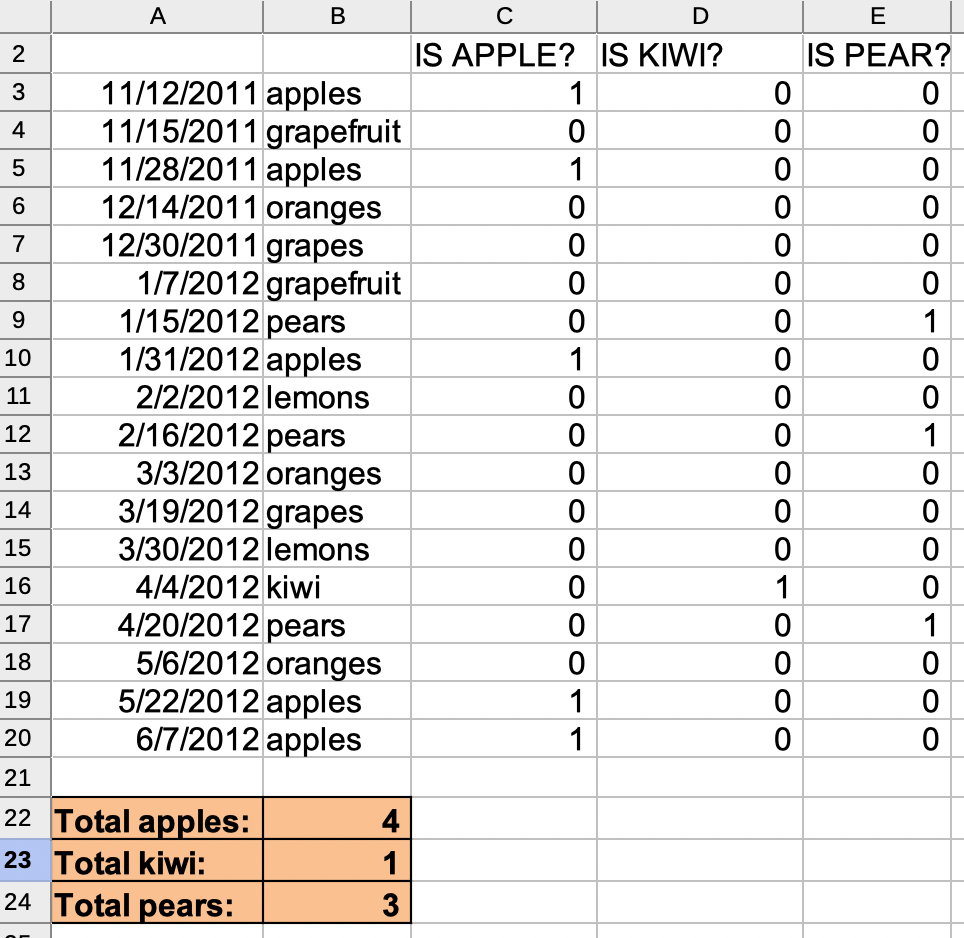
\includegraphics[width=0.9\textwidth]{Exercise3Soln.png}
	\end{center}
	\end{frame}
 
	\begin{frame}
		\frametitle{The Poisson Distribution}
	\end{frame}
	\begin{frame}
		\frametitle{The POISSON() Function}
	\end{frame}
	\begin{frame}
		\frametitle{Example: Counting Train Arrivals}
	\end{frame}
	\begin{frame}
		\frametitle{Exercise 4: Hospital Supply Quality Control}
		A hospital supply room manager found that on average about 2 gloves in a box are not usable.
		 
		\begin{enumerate}
			\item Graph the probability and cumulative distributions for the Poisson distribution function with $\lambda = 2$ 
			\item Set the probability/cumulative outputs as a number with 4 decimal places.
			\item Experiment to see how many scores are needed to capture the sample space for the Poisson distribution function with $\lambda=2$. 
			\item Compute the following probabilities:
				\begin{itemize}
					\item Only $1$ glove will be unusable.
					\item Fewer than $5$ gloves will be unusable.
					\item At least $2$ gloves will be unusable.
				\end{itemize}
		\end{enumerate}
	\end{frame}
	\begin{frame}
		\frametitle{Exercise 4: Solution}
	\end{frame}
	\begin{frame}
		\frametitle{Further Reading}
		The topics covered in the lecture can be found in \textit{Compter Applications for Life Sciences} p. 63 - 74.
	\end{frame}
\end{document}
